\documentclass{article}
% \usepackage{hyperref}

\usepackage{titlesec}
\usepackage{titling}
\usepackage{multicol}
% \usepackage{hyperref}
\usepackage[margin=0.3in]{geometry}

\usepackage{MnSymbol}
\usepackage{amsmath} 
\usepackage{graphicx} 
\usepackage{eso-pic}
\usepackage[hidelinks]{hyperref}

\titleformat{\section}
{\large\uppercase}
{}
{0em}
{}[\titlerule]

\titleformat{\subsection}[runin]
{\bfseries}
{}
{1em}
{}[]

\renewcommand{\maketitle}{
    \begin{flushleft}        
        {\huge\rmfamily
        \theauthor}\newline
        \vspace{0.1em}
        \textit{teetangh@gmail.com -- github.com/teetangh}\newline
        \textit{Contact No. -- +91-8800441954}\newline
        \textit{Manipal Institute of Technology}\newline
        \textit{B.Tech in \textbf{Computer Science \& Engineering}}
        \textit{2018 - 2022}\newline
        \textit{Minor in \textbf{Computational Intelligence}}\newline
        \textit{CGPA: 8.45/10}\newline
    \end{flushleft}

}


\titlespacing*{\subsection}
{0em}
{0em}
{0em}


%%%%%%%%%%%%%%%%%%%%%%%%%%%%%%%%%%%%%%   DOCUMENT  %%%%%%%%%%%%%%%%%%%%%%%%%%%%%%%%%%%%%%%%%%%%%%%%%%%%%%%


\begin{document}
\thispagestyle{empty}  % for no page numbering

% \begin{multicols}{2}
%     \title{Resume}
%     \author{Kaustav Ghosh}
%     \maketitle
%     \begin{flushright}
%         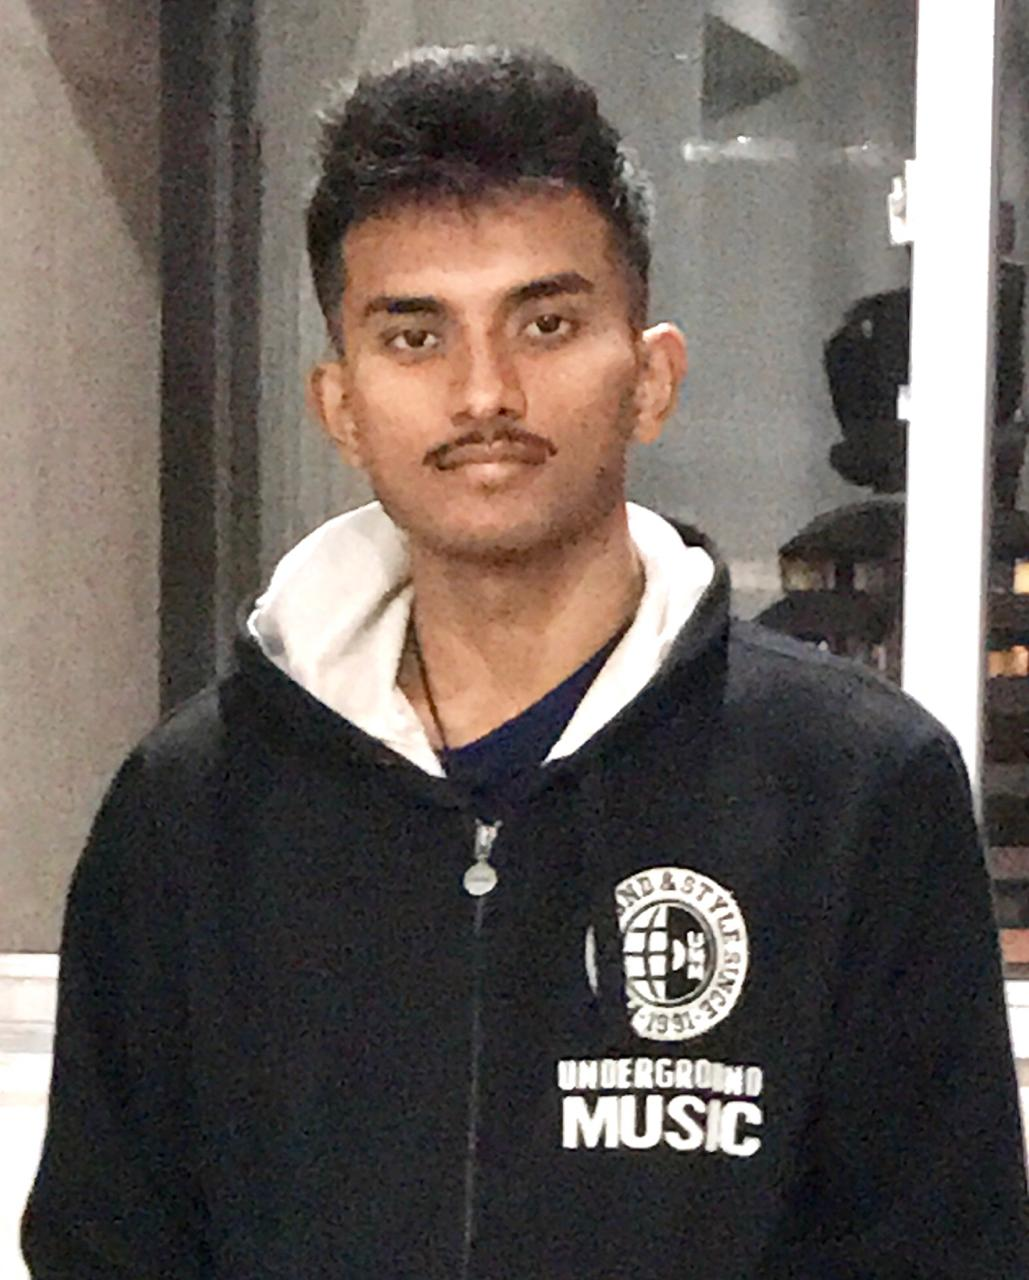
\includegraphics[height=3cm]{kaustav2.jpeg}
%     \end{flushright}
% \end{multicols}

\begin{center}
    \huge{Kaustav Ghosh}

    \normalsize{
        \textit{
            +91-8800441954 \(|\)
            teetangh@gmail.com \(|\)
            \href{https://www.github.com/teetangh}{GitHub} \(|\)
            \href{https://www.linkedin.com/in/kaustav-ghosh-1538651bb/}{LinkedIn} \(|\)
            Gugraon,India
        }}
\end{center}

\section*{Education}
% \subsection*{
%     Manipal Institute of Technology
%     \begin{flushright}
%         \text{2018-2022}
%     \end{flushright}
%     }

% Left \hfill Center \hfill Right
\textbf{Manipal Institute of Technology} \hfill \textit{2018-2022}
\textmd{\newline \textit{BTech in Computer Science and Engineering specializing in Computational Intelligence}} \hfill \textit{CGPA: 8.45/10}
\textmd{\newline \textit{Interests: Artificial Intelligence and Robotics}}

\section*{Internships}

\begin{itemize}
    \item{\textbf{\large{Samsung Research, Bengaluru - IoT Products and Analytics Intern}}} \hfill \textit{Jun'21-Jul'21}
          \newline
          \textit{- Working on developing MQTT bridge functionality in Moquette, a lightweight Java MQTT broker}
\end{itemize}


\begin{itemize}
    \item{\textbf{\large{Microsoft Student Partners-Machine Learning Intern}}} \hfill \textit{Apr'20-Jun'20}
          \newline
          \textit{-Guided a team of 10 individuals to collaborate and accomplish a Regression task of price prediction of used cars in a machine learning pipeline through Exploratory Data Analysis,Feature Engineering and Model Building.}
          % \newline
          % \textit{- Guided a team of 10 individuals to collaborate and accomplish a Regression task of price prediction of used cars}
          % \newline
          % \textit{- Performed Feature Engineering to detect the most important attributes of the data-set using Uni-variate and Multivariate Filtering techniques, Mutual Entropy Gain Filtering and also feature selection using RMSE Regression and ANOVA Test  }
          % \newline
          % \textit{- Performed basic Data wrangling and processing using numpy and pandas and visualized it using matplotlib and seaborn and finally built the machine learning model using an XGboost Regressor }
          % \newline
          % \textit{- Also completed a Mini Project on extensive Data Visualization and Analysis using Matplotlib and Seaborn to gather useful insights of the data}
          % % \newline
          % % \textbf{ Mini Project:} \href{https://github.com/teetangh/Microsoft-Machine-Learning-Internship/blob/master/MINOR%20PROJECT/Microsoft_Minor_Project_v2.ipynb}{Notebook}.
\end{itemize}

\begin{itemize}
    \item{\textbf{\large{Qbotics Labs - ROS Engineer Intern}}}\hfill \textit{Jul'20-Aug'20}
          \newline
          \textit{- Constructed a Differential Drive with caster wheel from scratch using URDF and XACRO files and mounted the same with laser scanner , IMU and Velodyne Puck VLP-16 Lidar and simulated the same in Gazebo and Webots}
          % \newline
          % \textit{- Constructed a Differential Drive with caster wheel from scratch using URDF and XACRO files and mounted the same with laser scanner , Inertial Measurement Unit and Velodyne Puck VLP-16 Lidar. }
          % \newline
          % \textit{- Simulated the differential drive in \underline{Gazebo} and wrote ROS Subscriber script to get laser scan reading from sensor messages for obstacle range detection }
          % \newline
          % \textit{- Interfaced the differential drive with \underline{Google Cartographer} with localisation and mapping of the robot using lua config files. }
          % % \newline
          % % \textit{Currently working on motion planning(including obstacle avoidance and wallflower)}
          % \newline
          % \textit{- Modelled a 4 wheeled drive and also an environment for experimentation of various controllers for the vehicle in \underline{Webots 3D Robot Simulator}}
          % \newline
          % \textit{- Wrote individual C++ controllers for the teleoperation using keyboard,laser scanner,GPS,IMU and Linear Actuator}
          % \newline
          % \textit{- Wrote \underline{Markdown documentation} for the entirety of the Internship for beginners to understand concepts and replicate results}
\end{itemize}


% \begin{itemize}
%     \item{\textbf{\large{United Nations TakenMind - Data Analytics Intern}}}
%           \newline
%           \textit{- Performed Exploratory Data Analysis techniques using Matplotlib and
%               Implemented several boxplots,countplots,heatmaps on several data-sets using Seaborn }
% \end{itemize}


% \begin{itemize}
%     \item{\textbf{\large{Ineuron Deep Learning with Masters in Computer Vision and Natural Language Processing}}}
%           \newline
%           \textit{- Postponed due to Covid Situation }
% \end{itemize}

\section*{Research Projects}
\begin{itemize}
    \item{\textbf{\large{Samsung PRISM - Intelligent Ranking for Dynamic Restoration in
                  Next Generation Wireless Networks}}} \hfill \textit{Sep'20-Mar'21}
          \newline
          \textit{- Implemented Machine Learning algorithms and Feature Engineering techniques to predict KPI values for eNodeB-s and consequently a ranking system
              to orderly restore them during network failure.}
\end{itemize}

\section*{Academic Projects}
\begin{itemize}
    \item{\textbf{\large{Compiler Frontend for subset of C-Language}}}
          % Don't know why indentation is not working
          \newline
          \textit{- Coded a \textbf{Lexical Analyser} that extracts tokens from a C source file and a \textbf{Symbol Table Generator} to store information of identifiers and functions and a \textbf{Recursive Decent Parser} that semantically parses the grammar for subset of C-Language by analysing the tokens generated by a Lexical Analyser}

    \item{\textbf{\large{Mini Games based on Backtracking}}}
          \newline
          \textit{- Coded a \textbf{Crossword Solver} that takes a 10*10 grid and word list and outputs a grid with the words accurately filled}
          \newline
          \textit{- Coded a \textbf{Sudoku Solver} that takes a partially filled 9*9 Sudoku grid and outputs a solution so that every row, column and nine 3x3 sub-grids contains exactly 1 instance of the digits from 1 to 9.}

    \item{\textbf{\large{Machine Learning Algorithm Implementations}}}
          \newline
          \textit{- Implemented basic machine learning algorithms such as Linear Regression, K-Nearest Neighbours, Logistic Regression,K-Means Clustering from scratch without existing machine learning libraries.Currently implementing gradient descent algorthims}


    \item{\textbf{\large{Covid 19 Time Series Forecasting, Data Analysis and Web Scraping}}}
          % Don't know why indentation is not working
          \newline
          \textit{- Prepared a complete Data Analysis report on the World-wide COVID-19 attack statistics and used the Facebook's fbprophet Time-series Forecasting library to speculate the number of active corona victim cases in the upcoming days.}
          % \newline
          % \textit{- Also used a corona dataset of my country and the Python folium package for the binding of data to a map for choropleth visualizations. Further used beautifulSoup and Requests HTTP library for Web Scraping of live corona stats.}
          % \newline
          % \textit{- Implemented code snippets for the pre-processing of data, data wrangling and visualized the data via several Matplotlib and Seaborn tools }
          % \newline
          % \textit{- Created neural networks from scratch which facilitated in implementing a machine learning model to recognize the function of an XOR gate without explicitly being programmed.}
          % \newline
          % \textit{- Trained a Deep Learning model using Tensorflow and Keras API for MNIST Handwritten digit Recognition}

          %\item{\textbf{\large{Data Exchange in Heterogeneous Systems}}}
          %\newline
          %\textit{- Learnt basic Fortran to script a Sine Series expansion, to import theta values \& export Sine theta values.}
          %\newline
          %\textit{- Used Java to import the same theta values \& export Cosine theta and store the same in MySQL database.}
          %\newline
          %\textit{- Used Python to import the Sine and Cosine thetas values to prove $\sin{^2\theta} + \cos{^2\theta} = 1$ }




    \item{\textbf{\large{Food Labs Robotics Startup Competition}}}
          \newline
          \textit{- Designed, modelled, constructed and
              Assembled a plethora of sensors and Robots across multiple software platforms like
              freeCad, Blender, Gazebo and also fabricated a Defense Building from scratch using floor plan and Gazebo World Editor}

          % \newline
          % \textit{- Created an SDF model of the Velodyne HDL-32 sensor,improved the model's appearance and data output,added Mass/Inertia to the model,used freeCad software to acquire Meshes, Blendr software to refine the metric system and Gazebo model editor to model the Velodyne Lidar structure.}
          % \newline
          % \textit{- Implemented Hokuyo Fake Laser Scanner and Noisy Camera in Gazebo, tweaked the mean and standard deviation of the Gaussian Noise Distribution in the scan and image samples for higher fidelity outputs.}
          % \newline
          % \textit{- Simulated the ROBOTIS waffle-pi or burger TurtleBot3 and constructed a vehicle in Gazebo using Model editor and loaded it with a Depth Camera Sensor for surveillance}
          % \newline



    \item{\textbf{\large{Analysis of Selective Compliance Assembly Robot Arm and Modelling of T3R Robot}}}
          \newline
          \textit{- Computed DH parameters for the SCARA robot and used it to compute the Forward and Inverse Kinematics of the robot arm and also its Lagrange Euler Dynamics}


          % \newline
          % \textit{- Computed Denavit–Hartenberg parameters for the SCARA robot and used it to formulate the Forward and Inverse Kinematics of the robot arm} 
          % \newline
          % \textit{- Used Lagrange Euler Formulation to compute the torque/dynamics of the robot and further also planned an arbitrary trajectory for the manipulator} 
          % \newline
          % \textit{- Using Solidworks modelled a T3R robot (1 twisting joint and 3 revolute joints) and as bonus task i am trying to interface the Solidworks model with Matlab Simscape}
\end{itemize}


% \section*{Positions of Responsibility}
% \textmd{Local Committee Member of IOSD(International Organization of Software Developers)}

% \section{Courses Taken}
% % \subsection*{}
% \textbf{Coding Ninjas}- Completed C++ \& Data Structures.Currently doing Algorithms \& Competitive Programming Course.
% \newline
% \textbf{NPTEL}-Basic Electronics,Switching Circuits \& Logic Design,Computer Organization \& Architecture,OOP with Java

\section*{Technical Section}
\subsection*{Softwares Used:}
AutoCAD,Matlab,Keil,Altera MaxPlus 2,VirtualBox,Vm Ware,Oracle SQL,GNS 3 Network Simulator
\subsection*{Programming Languages:}
Fluent in C/C++ \& Python ,Familiar with Java ,Verilog,{\LaTeX},Linux Shell Scripting,
fair acquaintance with ARM assembly programming\textit{(NXP LPC 1768)}
\subsection*{Libraries \& Frameworks:}
\textbf{C++}-STL
\textbf{Java}-JavaFX GUI
\textbf{Python}-Numpy, Pandas, Scikit-Learn, Keras, Tensorflow , PyTorch
% \subsection*{Robotics Libraries \& Frameworks:}
% ROS middleware, Gazebo, Ignition, MoveIt!, Point Cloud Library
%\subsection*{Web-Dev Languages,Libraries \& Frameworks:}
%Fair acquaintance with HTML, CSS, JavaScript \& with MERN %stack
\subsection*{Operating Systems Used:}
\textbf{Windows}-XP,Vista,7,10
\textbf{Linux}-Ubuntu
\end{document}